% \newprob{1715575628}
% {
%     下列有關在繩子中傳播的波的敘述,哪項是\textbf{不正確}的?\\Which of the following statements about propagation of waves is \textbf{incorrect}?
%     \begin{tasks}
%         \task 波由振動源產生。\\Wave is generated by oscillating source.
%         \task 每個粒子都圍繞各自的平衡位置振動。
%         \task 粒子的位移到達最大值時,能量為零。
%         \task 能量會在相鄰粒子之間傳遞。
%     \end{tasks}

% }{
%     \mckey C
% }


\newprob{1715587302}
{
    下圖顯示一個拉長了的軟彈簧。\\The figure below shows a stretched spring.
    \par{\par\centering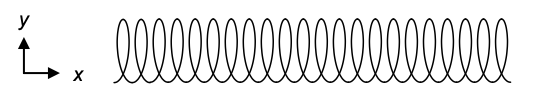
\includegraphics[width=.4\textwidth]{./img/ch1_earlyclass_wave_mc_2024-05-13-16-02-17.png}\par}
    下列哪些敘述是正確的?\\Which of the following statements are correct?
    \begin{statements}
        \task 如果一列縱波沿彈簧傳播,彈簧圈會沿方向x振動。\\If a longitudinal wave propagates along a spring, the coils of the spring will vibrate in the x-direction.
        \task 如果一列橫波沿彈簧傳播,能量會沿方向x傳播。\\If a transverse wave propagates along a spring, the energy will be transmitted in the x-direction.
        \task 一個振動源可同時產生橫波和縱波。\\A vibrating source can simultaneously generate both transverse and longitudinal waves.
    \end{statements}
    \begin{tasks}
        \task 只有(1)和(2) \tab\tab (1) and (2) only
        \task 只有(1)和(3) \tab\tab (1) and (3) only
        \task 只有(2)和(3) \tab\tab (2) and (3) only
        \task (1), (2) 和 (3)\tab\tab (1), (2) and (3)
    \end{tasks}

}{D}


\newprob{1715587507}
{
    下圖顯示一列橫向行波。如果處於A的波峯傳播到B需時3 s,波的速率和頻率是多少?\\The figure below shows a transverse traveling wave. If it takes 3 s for the wave peak at point A to propagate to point B, what is the velocity and frequency of the wave?
    \par{\par\centering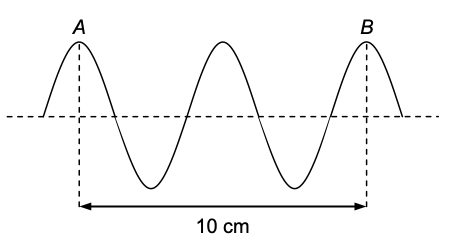
\includegraphics[width=.4\textwidth]{./img/ch1_earlyclass_wave_mc_2024-05-13-16-05-45.png}\par}
    \begin{tasks}
        \task [] \textbf{速率 speed /m s}$\mathbf{^{-1}}$ \tab \textbf{頻率 freq /Hz}
        \task 0.0167 \tab\tab 0.333
        \task 0.0167 \tab\tab 0.0167
        \task 0.0333 \tab\tab 0.667
        \task 0.0333 \tab\tab 0.0166
    \end{tasks}

}{C}


\newprob{1715588106}
{
    下圖顯示一列縱波。\\The following figure shows a longitudinal wave.
    \par{\par\centering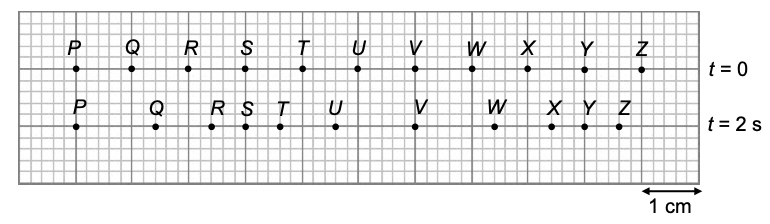
\includegraphics[width=.6\textwidth]{./img/ch1_earlyclass_wave_mc_2024-05-13-16-15-20.png}\par}
    下列哪對粒子的振動反相?\\Which of the following pair of particles are in antiphase?
    \begin{tasks}
        \task $P$和$V$
        \task $S$和$Y$
        \task $R$和$T$
        \task $V$和$Y$
    \end{tasks}

}{D}

\newprob{1715588215}
{
    下列哪項有關縱波的敘述是\textbf{不正確}的?\\Which of the following about longitudinal waves is \textbf{incorrect}?
    \begin{tasks}
        \task 所有聲波都是縱波。\\All sound waves are longitudinal.
        \task 處於密部中心的粒子是瞬間靜止的。\\The particles at the center of compression of the wave is momentarily at rest.
        \task 縱波上的所有粒子都帶有能量。\\All particles along the wave carry energy.
        \task 粒子沿波的傳播方向振動。\\The particles vibrate along the direction of wave propagation.
    \end{tasks}

}{B}

\newprob{1715588251}
{
    以下顯示一列縱波。\\The following shows a longitudinal wave.
    \par{\par\centering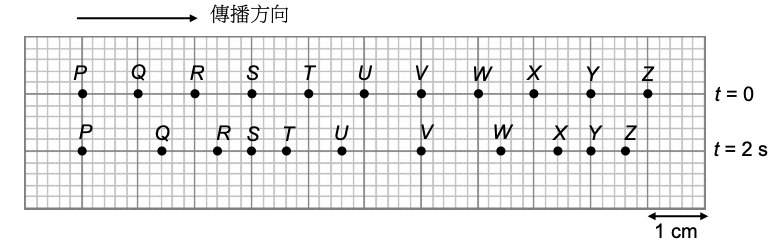
\includegraphics[width=.6\textwidth]{./img/ch1_earlyclass_wave_mc_2024-05-13-16-17-43.png}\par}
    在$t$ = 2 s時,$Q$和$Y$分別往哪個方向運動?\\At $t$ = 2 seconds, in which directions are $Q$ and $Y$ moving respectively?
    \begin{tasks}
        \task [] \textbf{Q} \tab\tab \textbf{Y}
        \task $\leftarrow$ \tab\tab $\leftarrow$
        \task $\leftarrow$ \tab\tab $\rightarrow$
        \task $\rightarrow$ \tab\tab $\leftarrow$
        \task $\rightarrow$ \tab\tab $\rightarrow$
    \end{tasks}
}{B}

\newprob{1715588357}
{
    如圖所示,一支 659 Hz 的音叉敲擊後發出聲波。已知聲音在空氣中的波長是 \vel{330}。\\As shown in the diagram, a 659 Hz tuning fork produces a sound wave when struck. It is known that the wavelength of sound in air is \vel{330}.
    \par{\par\centering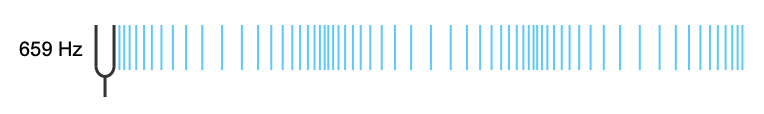
\includegraphics[width=.6\textwidth]{./img/ch1_earlyclass_wave_mc_2024-05-13-16-20-01.png}\par}
    兩個相鄰密部之間的距離是多少?\\What is the distance between neighboring compression?

    \begin{tasks}
        \task 0.25 m
        \task 0.50 m
        \task 0.75 m
        \task 1.00 m
    \end{tasks}

}{B}

\newprob{1715588462}
{
    一列縱波以速率 \vel{3000}在某介質中傳播。以下顯示介質中一個粒子的位移—時間關係線圖,取波的傳播方向為正。\\A longitudinal wave propagates through a certain medium with a velocity of \vel{3000}. The diagram below shows the displacement-time relationship of a particle in the medium, with the direction of wave propagation taken as positive.
    \par{\par\centering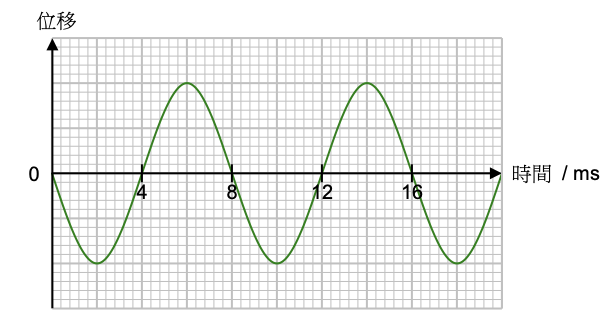
\includegraphics[width=.5\textwidth]{./img/ch1_earlyclass_wave_mc_2024-05-13-16-21-19.png}\par}
    粒子在甚麼時間處於疏部中心?\\What time is the particle located at  in the center of rarefraction?
    \begin{tasks}
        \task $t=4$ \unit{m.s}
        \task $t=6$ \unit{m.s}
        \task $t=8$ \unit{m.s}
        \task $t=10$ \unit{m.s}
    \end{tasks}


}{C}

\newprob{1715588559}
{
    以下顯示一列向右傳播縱波的位移—距離關係線圖,取向右為正。\\The following graph shows the displacement-distance relationship of a longitudinal wave propagating to the right, where positive direction is taken to the right.
    \par{\par\centering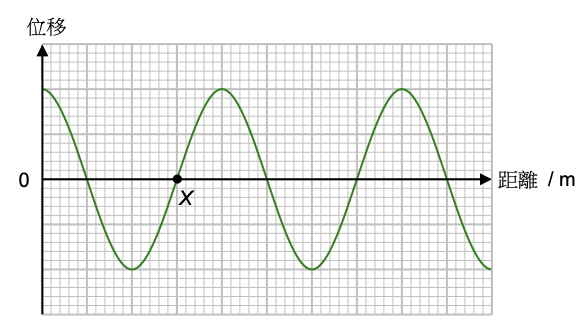
\includegraphics[width=.5\textwidth]{./img/ch1_earlyclass_wave_mc_2024-05-13-16-22-56.png}\par}
    下列哪項有關$X$的敘述是\textbf{不正確}的?\\Which of the following statements about $X$ is \textbf{incorrect}?
    \begin{tasks}
        \task $X$正處於疏部中心。\\$X$ is located at center of rarefraction.
            \task $X$正處於平衡位置。\\$X$ is loacted at equilibrium position.
            \task $X$正在向右移動。\\$X$ is moving towards the right.
            \task $X$正處於最大速率。\\$X$ is the at maximum speed.
    \end{tasks}

}{C}